\chapter{ASA Security Device Manager (ASDM)}

\section{Starting ASDM}

The Cisco ASA can be configured and managed using either the command line interface (CLI) or by using the graphical user interface (GUI) ASA Security Device Manager (ASDM). The CLI is fast but requires more time to learn while ASDM is intuitive and simplifies the ASA configuration. It works with SSL to ensure secure communication with the ASA. It also provides quick-configuration wizards and logging and monitoring functionality that is not available using the CLI.

\subsection{Password Recovery Procedure}

To recover passwords for the ASA, perform the following steps:

\begin{enumerate}
\item Connect to the ASA console port and restart the ASA (Power off, and then power it on).
\item After startup, press the Escape key when you are prompted to enter ROMMON mode.
\item In the ROMMON mode, enter the \code{confreg 0x41} command to update the configuration register value.
\item To set the ASA to ignore the startup configuration, enter \code{confreg}.
\end{enumerate}

\subsection{Preparing for ASDM}

To enable access to the ASDM, the ASA requires some minimal configurations. Specifically, to prepare for ASDM access on an ASA 5505, the following must be configured:

\begin{itemize}
\item Inside logical VLAN interface -- Assign the Layer 3 address and the security level.
\item Ethernet 0/1 physical port -- By default it is assigned to VLAN 1, but must be enabled.
\item Enable the ASA Web Server -- Disabled by default.
\item Permit access to the ASA Web Server -- By default, the ASA operates in a closed policy; therefore, all connections to the HTTP server are denied.
\end{itemize}

The example in Figure \ref{PrepareASA} configures the logical management inside interface with IP address 192.168.1.1. It enables Ethernet 0/1, enables the ASA HTTP server, and permits access from an inside host with IP address 192.168.1.3. To remove and disable the ASA HTTP server service, use the \code{clear configure http} global configuration mode command.

\begin{figure}[hbtp]
\caption{Preparing ASDM}\label{PrepareASA}
\centering
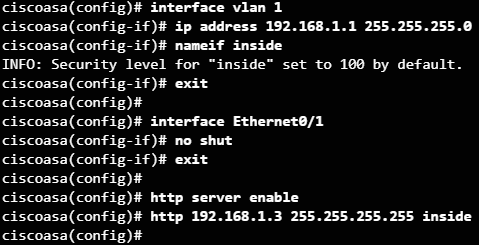
\includegraphics[scale=1]{pictures/PrepareASA.PNG}
\end{figure}

\subsection{Install ASDM}

To start ASDM, enter the management IP address of the ASA in a web browser from a PC. The ASDM launch window is displayed, as shown in Figure 2, providing two options:

\begin{itemize}
\item \textbf{Run Cisco ASDM as a local application} -- This provides the \textbf{Install ASDM Launcher} option to connect to the ASA from the host’s desktop using SSL. The advantage of doing so is that one application can be used to manage several ASA devices, and an Internet browser is not required to start ASDM.
\item \textbf{Run Cisco ASDM as a Java Web Start application} -- This provides the \textbf{Run ASDM} option to run the ASDM application. Using an Internet browser is required to establish a connection. ASDM is not installed on the local host. The Run Startup Wizard option can be selected instead. It provides a step-by-step initial configuration similar to the CLI Setup Initialization wizard.
\end{itemize}

In this example, \textbf{Run ASDM} is selected. If security warning appears, click \textbf{Continue}. Next a security warning is displayed stating that ASDM could be a security risk. Accept the risk and then click \textbf{Run}. ASDM then displays the Cisco ASDM-IDM Launcher. The launcher requests a username and password. Because none were initially configured, leave these fields blank and click \textbf{OK}.\\


Cisco ASDM offers several wizards to help simplify the configuration of the appliance:

\begin{itemize}
\item Startup Wizard: Modify existing configuration or to Reset configuration to factory defaults
\item VPN Wizards
\item Other wizard: High Availability and Scalability Wizard, Unified Communication Wizard, ASDM Identity Certificate Wizard, Packet Capture Wizard
\end{itemize}


\section{Basic configuration}

The ASDM Configuration view is required to configure most device settings using the following two main tabs:

\begin{itemize}
\item \textbf{Device Setup:} this tab can be used to configure the hostname, passwords, system time, interface settings, and routing.
\item \textbf{Device Management:} this tab can be used to configure management access, users and AAA access, DHCP, and more. Specifically, this tab can be used to configure basic management features including legal notification and to create a master passphrase.
\end{itemize}

Basic ASA settings include a device hostname, enable password, master passphrase, and banner. To configure the ASA hostname, domain name, and enable password, click Configuration > Device Setup > Device Name/Password. To configure a master passphrase and encrypt all passwords, click Configuration > Device Management > Advanced > Master Passphrase. On this page, the master passphrase can be created and enabled to use AES encryption. To configure legal notification, click Configuration > Device Management > Management Access > Command Line (CLI) > Banner. On this page, various banners can be created and edited.



\subsection{Basic settings}



\section{Advanced configuration}